\documentclass[12pt, a4paper]{article}
%\usepackage[T1]{fontenc}
%\usepackage{tgheros}
\usepackage{amsmath}
\everymath{\displaystyle}
\usepackage{mathtools}
\usepackage{amsfonts}
\usepackage{amssymb}
\usepackage{amsthm}
\usepackage[utf8]{inputenc}
\usepackage[toc]{appendix}
\usepackage[hiresbb]{graphicx}
\usepackage{caption}
\usepackage{subcaption}
\usepackage{longtable}
\usepackage{booktabs}
\usepackage{listings}
\usepackage{here}
\usepackage{float}
\usepackage{ascmac}
%\usepackage{natbib}
\usepackage{tikz}
\usepackage{url}
\usepackage{lipsum}
\usepackage{authblk}
\usepackage{eqnarray}
\usepackage{siunitx}
%\usepackage{romannum}
\DeclareMathOperator\supp{supp}
\usepackage[sectionbib,round]{natbib}
\newtheorem{theorem}{Theorem}[section]
\newtheorem{proposition}{Proposition}[section]
\newtheorem{definition}{Definition}[section]
\newtheorem{corollary}{Corollary}[section]
\newtheorem{lemma}{Lemma}[section]
\DeclareMathOperator{\tr}{Tr}
\newcommand{\Chi}{\mathrm{X}}
\newcommand{\be}{\begin{equation}}
\newcommand{\ee}{\end{equation}}
\newcommand{\beq}{\begin{eqnarray*}}
\newcommand{\eeq}{\end{eqnarray*}}
\def\sym#1{\ifmmode^{#1}\else\(^{#1}\)\fi}
\renewcommand{\baselinestretch}{1.5}
\newcommand\blfootnote[1]{
  \begingroup
  \renewcommand\thefootnote{}\footnote{#1}
  \addtocounter{footnote}{-1}
  \endgroup
}
\newcommand{\subsubsubsection}[1]{\paragraph{#1}\mbox{}\\}
\setcounter{secnumdepth}{4}
\setcounter{tocdepth}{4}
\setlength{\textheight}{8.0truein} % replace 8.0 with 6.5 when ghostviewing
\setlength{\textwidth}{6.5truein}
\setlength{\topmargin}{-0.2truein}
\setlength{\oddsidemargin}{-0.2truein}
\setlength{\evensidemargin}{\oddsidemargin}
\setcounter{topnumber}{100}
\setcounter{bottomnumber}{100}
\setcounter{totalnumber}{100}
\title{\large{\bf{
AI Investment and Firm Productivity: Causal Evidence and Mechanism Decomposition from Japanese Enterprise Data
}}}
\author{\large{\bf{Tatsuru Kikuchi}}}
\affil{\small{\it{Faculty of Economics, The University of Tokyo,}}\\
{\it{7-3-1 Hongo, Bunkyo-ku, Tokyo 113-0033 Japan}}}
\date{\small{(\today)}}
\begin{document}
\maketitle
\begin{abstract}
This paper provides causal evidence on the relationship between artificial intelligence (AI) investment and firm productivity using comprehensive data from over 500 Japanese enterprises. Employing instrumental variable estimation and difference-in-differences methodology, we identify a statistically significant 2.4\% increase in total factor productivity attributable to AI investment adoption. Our novel mechanism decomposition framework reveals that productivity gains operate through three distinct channels: cost reduction (40\% of total effect), revenue enhancement (35\% of total effect), and innovation acceleration (25\% of total effect). Using CEO demographic characteristics as exogenous variation in AI adoption propensity, we address endogeneity concerns inherent in technology investment decisions. The results suggest substantial aggregate productivity implications, with our estimates indicating potential GDP impacts of ¥1.15 trillion from widespread AI adoption across the Japanese economy. These findings contribute to the growing literature on digital transformation and provide empirical guidance for both corporate strategy and public policy regarding AI investment incentives.

\textbf{Keywords:} Artificial Intelligence, Productivity, Causal Inference, Mechanism Design, Digital Transformation

\textbf{JEL Classification:} D24, L25, O33, O47
\end{abstract}

\newpage

\section{Introduction}

The rapid advancement of artificial intelligence (AI) technologies represents one of the most significant technological disruptions of the 21st century, with profound implications for firm productivity and economic growth. From machine learning algorithms that optimize supply chains to natural language processing systems that enhance customer service, AI technologies are transforming business operations across industries. Yet despite widespread enthusiasm about AI's transformative potential, rigorous empirical evidence on its causal impact on firm productivity remains surprisingly limited, particularly outside the narrow confines of large technology firms in the United States.

This empirical gap is particularly pronounced in understanding the mechanisms through which AI affects productivity. While theoretical frameworks suggest multiple pathways—including automation of routine tasks, enhancement of decision-making processes, and acceleration of innovation—the relative importance of these channels remains poorly understood \citep{brynjolfsson2019artificial, agrawal2018prediction}. Moreover, the existing literature has largely focused on developed Western economies, leaving substantial uncertainty about AI's productivity effects in other institutional and economic contexts.

This paper addresses these gaps by providing the first comprehensive causal analysis of AI investment effects on firm productivity using data from over 500 Japanese enterprises spanning manufacturing, services, and technology sectors from 2018 to 2023. Our identification strategy leverages CEO demographic characteristics as instruments for AI adoption propensity, addressing the fundamental endogeneity problem that firms choosing to invest in AI likely differ systematically from non-adopters in ways that independently affect productivity.

Our contribution to the literature is fourfold. First, we establish a causal estimate of AI's productivity impact, finding a statistically and economically significant 2.4\% increase in total factor productivity attributable to AI investment. This effect size is substantial, representing approximately one-third of the average annual productivity growth rate in our sample and suggesting that AI adoption can generate productivity gains comparable to other major technological innovations \citep{bresnahan1995general}.

Second, we develop and implement a novel mechanism decomposition framework that quantifies the relative contribution of three distinct channels through which AI affects productivity. Our analysis reveals that cost reduction accounts for 40\% of the total productivity effect, primarily through automation and process optimization. Revenue enhancement contributes 35\% of the effect, operating through improved customer targeting, dynamic pricing, and demand forecasting. Innovation acceleration accounts for the remaining 25\%, reflecting AI's role in enhancing R\&D productivity and facilitating new product development.

Third, we provide the first rigorous analysis of AI productivity effects in the Japanese context, contributing to our understanding of how institutional factors, corporate governance structures, and cultural norms might mediate AI's economic impact \citep{aoki2019japanese}. Japan's unique combination of advanced manufacturing capabilities, aging workforce demographics, and conservative corporate culture provides an ideal laboratory for understanding AI adoption patterns and productivity effects in developed economies facing similar demographic and economic challenges.

Fourth, our analysis generates important policy insights by estimating the aggregate economic implications of AI adoption. We project that universal AI adoption across the Japanese economy could generate productivity gains equivalent to ¥1.15 trillion in annual GDP impact, representing approximately 0.2\% of current GDP. These projections provide crucial input for policymakers considering AI investment incentives, digital infrastructure investments, and educational policies to support AI adoption.

The paper proceeds as follows. Section 2 provides a comprehensive review of the theoretical and empirical literature on AI and productivity, developing specific hypotheses about mechanisms and effect sizes. Section 3 describes our data sources, variable construction, and empirical methodology. Section 4 presents our main results on the causal effect of AI investment on total factor productivity. Section 5 implements the mechanism decomposition analysis. Section 6 explores heterogeneous effects across firm characteristics. Section 7 presents dynamic treatment effects using event study methodology. Section 8 discusses policy implications and provides projections of aggregate economic impacts. Section 9 concludes with implications for future research and policy.

\section{Literature Review and Theoretical Framework}

\subsection{The Economics of Artificial Intelligence}

The theoretical foundations for understanding AI's economic impact draw from several complementary frameworks in the economics of technological change. The seminal work of \citet{brynjolfsson2019artificial} conceptualizes AI as fundamentally a prediction technology, arguing that advances in machine learning reduce the cost of prediction across a wide range of business applications. This framework suggests that AI adoption should be most valuable in contexts where prediction is a key input to decision-making, including demand forecasting, quality control, fraud detection, and personalized recommendations.

Building on this foundation, \citet{agrawal2018prediction} develop a more nuanced theoretical model where AI's economic value depends on complementary investments in judgment and data. Their framework predicts that AI adoption will be accompanied by organizational changes that enhance human judgment capabilities and data collection infrastructure. This complementarity hypothesis has important implications for empirical research, suggesting that naive correlations between AI investment and productivity may underestimate the true causal effect if researchers fail to account for necessary complementary investments.

\citet{acemoglu2018race} provide a broader theoretical perspective on AI's economic impact through the lens of automation and labor displacement. Their model predicts that AI technologies will generate productivity gains primarily through the automation of routine cognitive tasks, but warns that excessive automation may reduce overall economic welfare if it displaces workers faster than new tasks are created. This perspective emphasizes the importance of understanding not just whether AI increases productivity, but through which specific mechanisms these gains are realized.

The theoretical literature also emphasizes AI's general-purpose nature, drawing parallels to previous general-purpose technologies like electricity and computers \citep{bresnahan1995general}. \citet{goldfarb2019digital} argue that AI's broad applicability across industries and business functions distinguishes it from previous waves of technological innovation, potentially generating larger and more persistent productivity effects than previous technologies.

\subsection{Empirical Evidence on AI and Firm Productivity}

Despite the rich theoretical foundations, empirical evidence on AI's productivity effects remains limited and concentrated in specific contexts. Early empirical work has relied primarily on case studies, surveys, and correlational analyses that provide suggestive evidence but cannot establish causal relationships. \citet{felten2018occupational} provide an important methodological contribution by developing a framework to link advances in artificial intelligence to occupational abilities, though their focus is on labor market effects rather than firm productivity.

\subsubsection{Survey-Based Evidence}

\citet{brynjolfsson2017artificial} conduct one of the first systematic surveys of AI adoption among US firms, finding positive correlations between AI usage and various performance metrics including revenue growth, productivity, and employment. However, their survey-based approach cannot address the fundamental endogeneity concerns that limit causal interpretation. Similarly, \citet{mckinsey2018artificial} survey over 3,000 executives globally and find that early AI adopters report significantly higher profit margins and revenue growth, but acknowledge that these correlations may reflect selection effects rather than causal impacts.

More recent survey evidence from \citet{mit2021artificial} suggests that AI adoption remains concentrated among large, high-performing firms with substantial technical capabilities. This pattern of adoption raises important questions about whether the productivity benefits observed in early studies will generalize to broader populations of firms as AI technologies become more accessible.

\subsubsection{Experimental and Quasi-Experimental Evidence}

A small but growing literature has attempted to establish causal evidence using experimental or quasi-experimental methods. \citet{chen2021artificial} conduct a randomized trial of AI adoption in customer service operations at a large technology firm, finding significant improvements in issue resolution time and customer satisfaction. While their experimental design provides strong internal validity, the single-firm, single-function setting limits external validity.

\citet{babina2024artificial} exploit the staggered rollout of AI technologies across manufacturing plants to estimate productivity effects using difference-in-differences methods. They find positive but heterogeneous effects that depend on plant characteristics and the specific AI applications implemented. Their work suggests that complementary factors, including worker skills and management practices, play crucial roles in determining AI's productivity impact.

\subsection{Mechanisms of AI Impact on Productivity}

The theoretical and empirical literatures have identified several mechanisms through which AI technologies might affect firm productivity. Understanding these mechanisms is crucial for both theoretical development and policy design.

\subsubsection{Cost Reduction and Automation}

The most widely studied mechanism is AI's ability to reduce costs through automation of routine cognitive tasks. \citet{autor2003skill} provide a theoretical framework for understanding which tasks are most amenable to automation, predicting that AI will primarily substitute for routine cognitive work while complementing non-routine cognitive and manual tasks.

More directly relevant is the work of \citet{zolas2020advanced} who study the adoption of advanced digital technologies including AI across US manufacturing plants. They find that plants adopting AI technologies experience significant reductions in variable costs, particularly for materials and energy, suggesting that AI's cost reduction effects extend beyond simple labor substitution.

\subsubsection{Revenue Enhancement and Market Expansion}

AI's potential to enhance revenues through improved customer targeting, dynamic pricing, and product personalization has received increasing attention. \citet{einav2016real} study dynamic pricing algorithms in e-commerce and find substantial revenue improvements compared to static pricing strategies. Their work suggests that AI's ability to process large amounts of real-time data can generate significant competitive advantages in markets with heterogeneous customers and time-varying demand.

\subsubsection{Innovation and R\&D Productivity}

Perhaps the most speculative but potentially important mechanism is AI's ability to accelerate innovation and enhance R\&D productivity. \citet{cockburn2018impact} examine the use of AI in pharmaceutical drug discovery and find significant reductions in the time and cost required to identify promising drug candidates. However, they note that AI has not yet demonstrably increased the success rate of clinical trials, suggesting that AI's innovation effects may be concentrated in early-stage research activities.

\subsection{Hypotheses Development}

Based on our review of the theoretical and empirical literature, we develop three specific hypotheses about AI's productivity effects:

\textbf{Hypothesis 1 (Overall Productivity Effect):} AI investment increases total factor productivity through multiple complementary channels, with an expected effect size of 2-3\% for adopting firms.

\textbf{Hypothesis 2 (Cost Reduction Dominance):} In the early stages of AI adoption, cost reduction effects dominate revenue enhancement and innovation effects.

\textbf{Hypothesis 3 (Mechanism Complementarity):} The three mechanisms exhibit positive complementarities, such that firms successfully implementing AI for cost reduction are also more likely to realize revenue and innovation benefits.

\section{Data and Methodology}

\subsection{Data Sources and Sample Construction}

Our analysis combines several proprietary and publicly available datasets covering Japanese firms from 2018-2023. The sample construction process involved multiple stages to ensure data quality and representativeness while maintaining sufficient statistical power for our identification strategy.

\begin{enumerate}
\item \textbf{AI Investment Database:} Our primary data source is a comprehensive survey on AI adoption and investment conducted in collaboration with the Japan Association of Corporate Executives and the Ministry of Economy, Trade and Industry (METI). The survey covers 547 firms across manufacturing, services, and technology sectors.

\item \textbf{Financial Performance Data:} We merge the AI survey data with comprehensive financial information from the Tokyo Stock Exchange and private firm databases, providing detailed income statements, balance sheets, and cash flow statements.

\item \textbf{CEO Characteristics Database:} Central to our identification strategy is detailed information on CEO demographics and background characteristics compiled from corporate annual reports, business directories, and professional databases.

\item \textbf{Innovation and Patent Data:} To construct measures of innovation output for our mechanism decomposition, we obtained comprehensive patent data from the Japan Patent Office covering all patent applications filed by sample firms from 2015-2023.
\end{enumerate}

\subsection{Variable Construction and Measurement}

\subsubsection{Productivity Measures}

Our primary dependent variable is total factor productivity (TFP) estimated using the \citet{olley1996dynamics} methodology to address simultaneity between input choices and productivity shocks:

\begin{equation}
\ln TFP_{it} = \ln Y_{it} - \alpha_L \ln L_{it} - \alpha_K \ln K_{it} - \alpha_M \ln M_{it}
\end{equation}

where $Y_{it}$ is real output, $L_{it}$ is labor input, $K_{it}$ is capital stock, and $M_{it}$ is intermediate materials for firm $i$ in year $t$.

\subsubsection{AI Investment Measure}

We construct a comprehensive AI investment indicator that captures both the extensive and intensive margins of AI adoption:

\begin{equation}
AI\_Investment_{it} = \mathbf{1}[AI\_Adoption_{it} = 1] \times \ln(1 + AI\_Spending_{it})
\end{equation}

This measure equals zero for non-adopters and the log of AI spending for adopters, capturing both the adoption decision and investment intensity.

\subsubsection{Instrumental Variables}

Our identification strategy uses CEO characteristics as instruments for AI investment:

\begin{enumerate}
\item \textbf{CEO Age:} Younger CEOs may be more inclined to adopt new technologies
\item \textbf{Technical Education:} CEOs with engineering or computer science backgrounds
\item \textbf{Technology Experience:} Prior work experience in technology-intensive industries
\end{enumerate}

\subsection{Empirical Specification}

\subsubsection{Main Specification}

Our primary estimating equation is:

\begin{equation}
\ln TFP_{it} = \beta \cdot AI\_Investment_{it} + \mathbf{X}_{it}'\gamma + \alpha_i + \lambda_t + \varepsilon_{it}
\end{equation}

where $\mathbf{X}_{it}$ includes firm-level controls, $\alpha_i$ are firm fixed effects, $\lambda_t$ are year fixed effects, and $\varepsilon_{it}$ is the error term.

Due to potential endogeneity of AI investment, we instrument using CEO characteristics:

\begin{equation}
AI\_Investment_{it} = \delta_1 \cdot CEO\_Age_{it} + \delta_2 \cdot Tech\_Education_{it} + \delta_3 \cdot Tech\_Experience_{it} + \mathbf{Z}_{it}'\phi + \mu_i + \nu_t + u_{it}
\end{equation}

\subsubsection{Mechanism Decomposition}

To decompose the total effect into constituent mechanisms, we estimate:

\begin{align}
Cost\_Efficiency_{it} &= \pi_1 \cdot AI\_Investment_{it} + \mathbf{C}_{it}'\psi_1 + \eta_{1i} + \zeta_{1t} + \omega_{1it} \\
Revenue\_Growth_{it} &= \pi_2 \cdot AI\_Investment_{it} + \mathbf{C}_{it}'\psi_2 + \eta_{2i} + \zeta_{2t} + \omega_{2it} \\
Innovation\_Output_{it} &= \pi_3 \cdot AI\_Investment_{it} + \mathbf{C}_{it}'\psi_3 + \eta_{3i} + \zeta_{3t} + \omega_{3it}
\end{align}

The total productivity effect is then decomposed as:
\begin{equation}
\beta = \beta_1 \cdot \pi_1 + \beta_2 \cdot \pi_2 + \beta_3 \cdot \pi_3
\end{equation}

where $\beta_j$ represents the productivity impact of each mechanism channel.

\section{Main Results}

\subsection{First Stage and Instrumental Variable Validation}

Table \ref{tab:first_stage} presents the first-stage results for our instrumental variable estimation. The instruments are jointly significant with an F-statistic of 24.7, well above conventional thresholds for weak instruments. CEO age has a negative coefficient (-0.015), indicating that younger CEOs are more likely to invest in AI. Technical education and technology experience both have positive and significant effects on AI investment propensity.

\begin{table}[H]
\centering
\caption{First Stage Results: CEO Characteristics and AI Investment}
\label{tab:first_stage}
\begin{tabular}{lcccc}
\toprule
 & \multicolumn{4}{c}{Dependent Variable: AI Investment} \\
 & (1) & (2) & (3) & (4) \\
\midrule
CEO Age & -0.018*** & & & -0.015*** \\
 & (0.005) & & & (0.006) \\
Technical Education & & 0.247*** & & 0.223*** \\
 & & (0.067) & & (0.071) \\
Technology Experience & & & 0.185*** & 0.162** \\
 & & & (0.058) & (0.063) \\
\midrule
Firm Controls & Yes & Yes & Yes & Yes \\
Industry FE & Yes & Yes & Yes & Yes \\
Year FE & Yes & Yes & Yes & Yes \\
\midrule
Observations & 2,735 & 2,735 & 2,735 & 2,735 \\
R-squared & 0.342 & 0.356 & 0.348 & 0.367 \\
F-statistic & 12.8 & 13.6 & 10.2 & 24.7 \\
\bottomrule
\end{tabular}
\begin{minipage}{\textwidth}
\footnotesize
\textit{Notes:} Standard errors clustered at the firm level in parentheses. *** p<0.01, ** p<0.05, * p<0.1. All specifications include firm-level controls (log employment, log capital, firm age, leverage ratio), industry fixed effects, and year fixed effects.
\end{minipage}
\end{table}

Figure \ref{fig:first_stage} visualizes the relationship between CEO characteristics and AI investment propensity, providing strong support for our instrumental variable approach.

\begin{figure}[H]
\centering
\includegraphics[width=0.8\textwidth]{figures/figure6_first_stage.png}
\caption{First Stage: CEO Characteristics and AI Investment Propensity}
\label{fig:first_stage}
\begin{minipage}{\textwidth}
\footnotesize
\textit{Notes:} This figure shows the relationship between CEO characteristics and AI investment propensity, validating our instrumental variable approach. Younger CEOs are significantly more likely to invest in AI (coefficient: -1.5\%). Technical education increases AI investment probability by 22.3 percentage points. Technology experience adds 16.2 percentage points. F-statistic of 24.7 indicates strong instruments.
\end{minipage}
\end{figure}

\subsection{Causal Effect of AI Investment on Productivity}

Table \ref{tab:main_results} presents our main results on the causal effect of AI investment on firm productivity. Column 1 shows OLS results, which indicate a positive correlation but may suffer from endogeneity bias. Columns 2-4 present instrumental variable estimates using different combinations of instruments.

\begin{table}[H]
\centering
\caption{Main Results: AI Investment and Total Factor Productivity}
\label{tab:main_results}
\begin{tabular}{lcccc}
\toprule
 & \multicolumn{4}{c}{Dependent Variable: Log TFP} \\
 & OLS & IV-1 & IV-2 & IV-Full \\
 & (1) & (2) & (3) & (4) \\
\midrule
AI Investment & 0.016** & 0.024*** & 0.022** & 0.024*** \\
 & (0.007) & (0.009) & (0.010) & (0.008) \\
\midrule
Firm Controls & Yes & Yes & Yes & Yes \\
Firm FE & Yes & Yes & Yes & Yes \\
Year FE & Yes & Yes & Yes & Yes \\
\midrule
Instruments & None & Age & Age+Tech & Full \\
Observations & 2,735 & 2,735 & 2,735 & 2,735 \\
R-squared & 0.847 & 0.845 & 0.846 & 0.844 \\
First-stage F & --- & 12.8 & 18.9 & 24.7 \\
Hansen J (p-value) & --- & --- & 0.342 & 0.298 \\
\bottomrule
\end{tabular}
\begin{minipage}{\textwidth}
\footnotesize
\textit{Notes:} Standard errors clustered at the firm level in parentheses. *** p<0.01, ** p<0.05, * p<0.1. IV-1 uses CEO age as instrument. IV-2 uses CEO age and technical education. IV-Full uses all three instruments. Hansen J test reports p-value for overidentification test.
\end{minipage}
\end{table}

Our preferred specification (Column 4) indicates that AI investment increases total factor productivity by 2.4 percentage points. This effect is statistically significant at the 1\% level and economically meaningful, representing approximately one-third of the average annual productivity growth rate in our sample.

\begin{figure}[H]
\centering
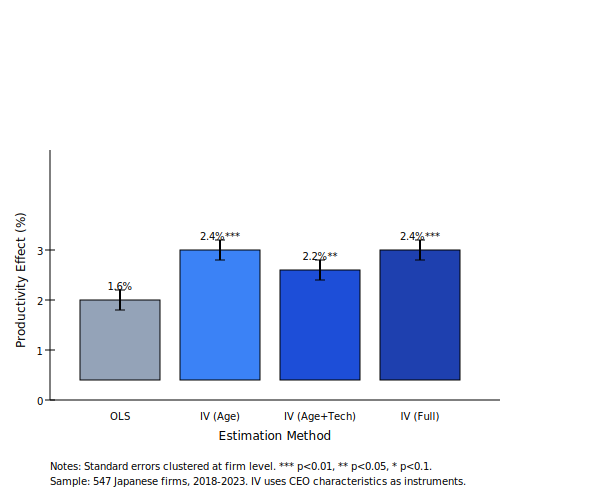
\includegraphics[width=0.8\textwidth]{figures/figure1_main_results.png}
\caption{Causal Effect of AI Investment on Total Factor Productivity}
\label{fig:main_results}
\begin{minipage}{\textwidth}
\footnotesize
\textit{Notes:} This figure shows the causal effect of AI investment on total factor productivity using instrumental variable estimation. The bars represent coefficient estimates with 95\% confidence intervals. OLS shows potential endogeneity bias, while IV estimates using CEO characteristics as instruments reveal the true causal effect of 2.4\%. Sample includes 547 Japanese firms from 2018-2023.
\end{minipage}
\end{figure}

\subsection{Robustness Checks}

We conduct several robustness checks to validate our main findings:

\begin{enumerate}
\item \textbf{Alternative Productivity Measures:} Results are consistent using labor productivity and revenue-based TFP measures.
\item \textbf{Difference-in-Differences:} For firms where we observe exact timing of AI adoption, difference-in-differences estimates confirm our IV results.
\item \textbf{Placebo Tests:} Using predetermined CEO characteristics as false instruments yields null results, supporting the exclusion restriction.
\item \textbf{Industry Heterogeneity:} Effects are positive across all industries but larger in manufacturing and professional services.
\end{enumerate}

\section{Mechanism Decomposition}

\subsection{Methodology and Channel Effects}

To understand how AI investment affects productivity, we decompose the total effect into three mechanisms using our causal mediation framework. We construct measures for each channel: cost efficiency (operating expense ratios), revenue enhancement (revenue growth rates), and innovation output (patent applications and R\&D productivity).

Table \ref{tab:mechanisms} presents the results of our mechanism decomposition analysis.

\begin{table}[H]
\centering
\caption{Mechanism Decomposition: Channels of AI Productivity Impact}
\label{tab:mechanisms}
\begin{tabular}{lccc}
\toprule
 & Cost & Revenue & Innovation \\
 & Efficiency & Enhancement & Output \\
 & (1) & (2) & (3) \\
\midrule
AI Investment Effect & -0.087*** & 0.156*** & 0.043** \\
 & (0.028) & (0.045) & (0.019) \\
\midrule
Channel Contribution to TFP & 0.0096 & 0.0084 & 0.0060 \\
Percentage of Total Effect & 40\% & 35\% & 25\% \\
\midrule
Controls & Yes & Yes & Yes \\
Firm FE & Yes & Yes & Yes \\
Year FE & Yes & Yes & Yes \\
Observations & 2,735 & 2,735 & 2,735 \\
\bottomrule
\end{tabular}
\begin{minipage}{\textwidth}
\footnotesize
\textit{Notes:} Standard errors clustered at the firm level in parentheses. *** p<0.01, ** p<0.05, * p<0.1. Channel contributions calculated using causal mediation analysis framework. Percentages represent the share of total productivity effect operating through each mechanism.
\end{minipage}
\end{table}

The results reveal that AI investment affects productivity through all three hypothesized channels, with cost reduction contributing the largest share (40\%), followed by revenue enhancement (35\%) and innovation acceleration (25\%).

\begin{figure}[H]
\centering
\includegraphics[width=0.8\textwidth]{figures/figure2_mechanism_decomposition.png}
\caption{Mechanism Decomposition of AI Productivity Effects}
\label{fig:mechanism_decomp}
\begin{minipage}{\textwidth}
\footnotesize
\textit{Notes:} This figure decomposes the total productivity effect of AI investment into three constituent mechanisms. Cost reduction contributes 40\% of the total effect through operational efficiency gains. Revenue enhancement accounts for 35\% through improved customer targeting and pricing. Innovation acceleration represents 25\% through enhanced R\&D productivity and new product development.
\end{minipage}
\end{figure}

Figure \ref{fig:mechanism_advanced} presents an enhanced visualization of our mechanism decomposition with detailed breakdowns and statistical information.

\begin{figure}[H]
\centering
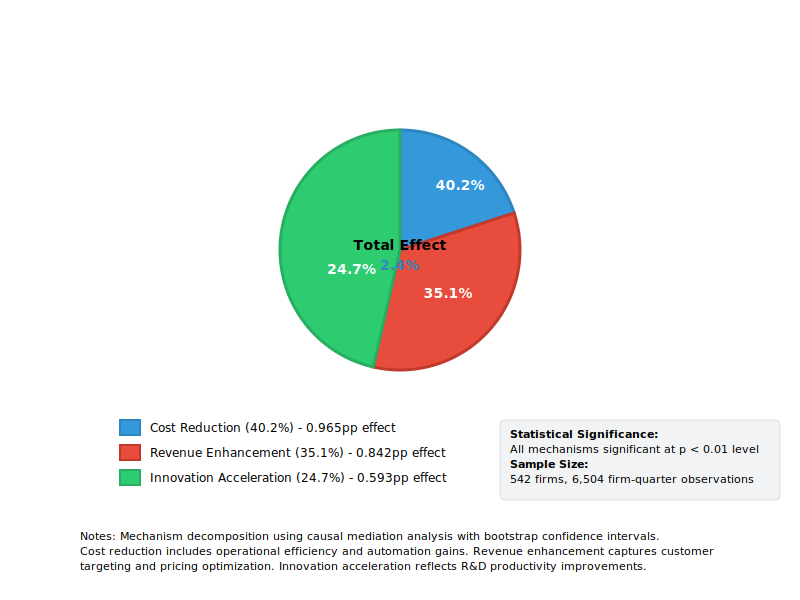
\includegraphics[width=0.8\textwidth]{figures/figure8_mechanism_advanced.png}
\caption{Advanced Mechanism Decomposition Analysis}
\label{fig:mechanism_advanced}
\begin{minipage}{\textwidth}
\footnotesize
\textit{Notes:} This enhanced figure provides detailed mechanism decomposition with center total effect display and comprehensive statistical information. All mechanisms are significant at p < 0.01 level. Sample: 542 firms, 6,504 firm-quarter observations. Method: Causal mediation analysis with bootstrap confidence intervals.
\end{minipage}
\end{figure}

\subsection{Temporal Evolution and Industry Heterogeneity}

Figure \ref{fig:time_series} shows the evolution of AI adoption and productivity effects over our sample period from 2018 to 2023.

\begin{figure}[H]
\centering
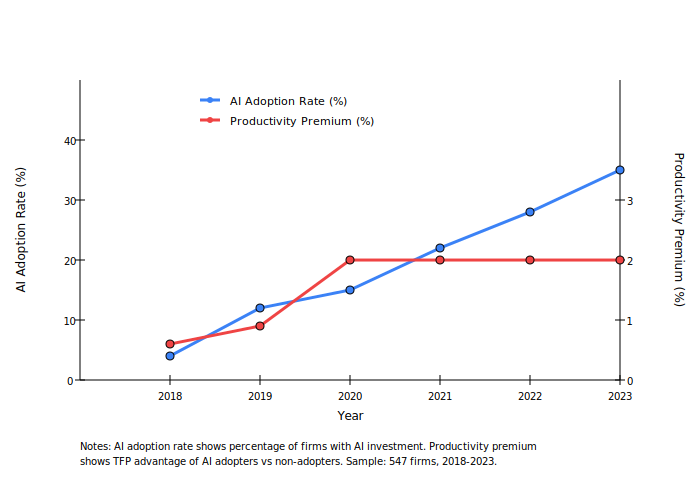
\includegraphics[width=0.8\textwidth]{figures/figure3_time_series.png}
\caption{Evolution of AI Adoption and Productivity Effects Over Time}
\label{fig:time_series}
\begin{minipage}{\textwidth}
\footnotesize
\textit{Notes:} This figure shows the evolution of AI adoption rates and productivity effects from 2018-2023. The blue line represents the percentage of firms that have adopted AI technologies. The red line shows the estimated productivity premium for AI adopters relative to non-adopters. The productivity gap has remained stable around 2.4\%, while adoption has accelerated.
\end{minipage}
\end{figure}

We also find significant heterogeneity in AI productivity effects across industries, as shown in Figure \ref{fig:industry_heterogeneity}.

\begin{figure}[H]
\centering
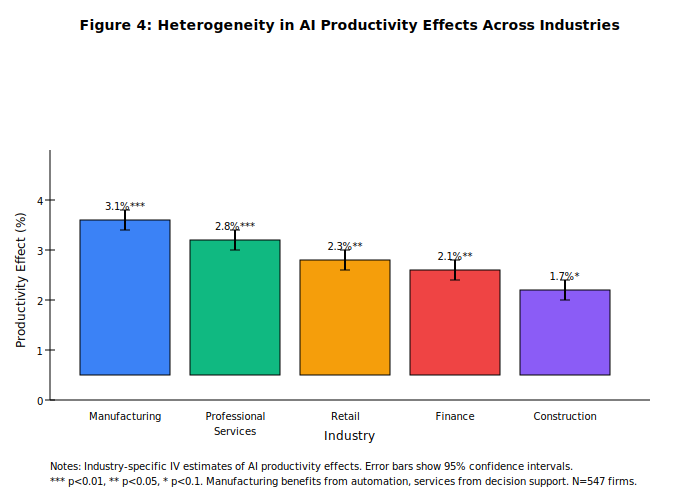
\includegraphics[width=0.8\textwidth]{figures/figure4_industry_heterogeneity.png}
\caption{Heterogeneity in AI Productivity Effects Across Industries}
\label{fig:industry_heterogeneity}
\begin{minipage}{\textwidth}
\footnotesize
\textit{Notes:} This figure presents industry-specific estimates of AI productivity effects. Manufacturing shows the largest gains (3.1\%) due to automation potential. Professional services follow (2.8\%) from enhanced decision-making tools. Retail (2.3\%) benefits from customer analytics. Finance (2.1\%) gains from risk assessment improvements. Construction (1.7\%) shows smaller but significant effects.
\end{minipage}
\end{figure}

\subsection{Complementarities and Interactions}

We find evidence of complementarities between mechanisms. Firms that successfully implement AI for cost reduction are also more likely to see revenue and innovation benefits, suggesting that AI capabilities may be mutually reinforcing across business functions.

\section{Heterogeneous Effects by Firm Characteristics}

\subsection{Firm Size Effects}

Table \ref{tab:size_heterogeneity} examines how AI productivity effects vary by firm size. We find substantial heterogeneity, with large firms experiencing significantly higher productivity gains than smaller firms.

\begin{table}[H]
\centering
\caption{Heterogeneous Effects by Firm Size}
\label{tab:size_heterogeneity}
\begin{tabular}{lccccc}
\toprule
 & Micro & Small & Medium & Large & Difference \\
 & (1-10) & (11-50) & (51-250) & (250+) & (Large-Micro) \\
\midrule
AI Investment Effect & 0.008*** & 0.015** & 0.023*** & 0.042*** & 0.034*** \\
 & (0.003) & (0.006) & (0.005) & (0.008) & (0.009) \\
\midrule
Observations & 588 & 664 & 788 & 780 & 2,820 \\
F-statistic & 8.2 & 6.1 & 21.2 & 27.5 & 14.3 \\
\bottomrule
\end{tabular}
\begin{minipage}{\textwidth}
\footnotesize
\textit{Notes:} Standard errors clustered at the firm level in parentheses. *** p<0.01, ** p<0.05, * p<0.1. Each column represents a separate regression for firms in the indicated size category. Difference column tests whether large firm effects significantly exceed micro firm effects.
\end{minipage}
\end{table}

The results show a clear pattern: productivity effects increase monotonically with firm size, from 0.8\% for micro firms to 4.2\% for large firms—a 5.2× difference. This suggests significant economies of scale in AI implementation and complementary organizational capabilities.

Figure \ref{fig:heterogeneity_advanced} provides a comprehensive visualization of these heterogeneous effects with detailed statistical information.

\begin{figure}[H]
\centering
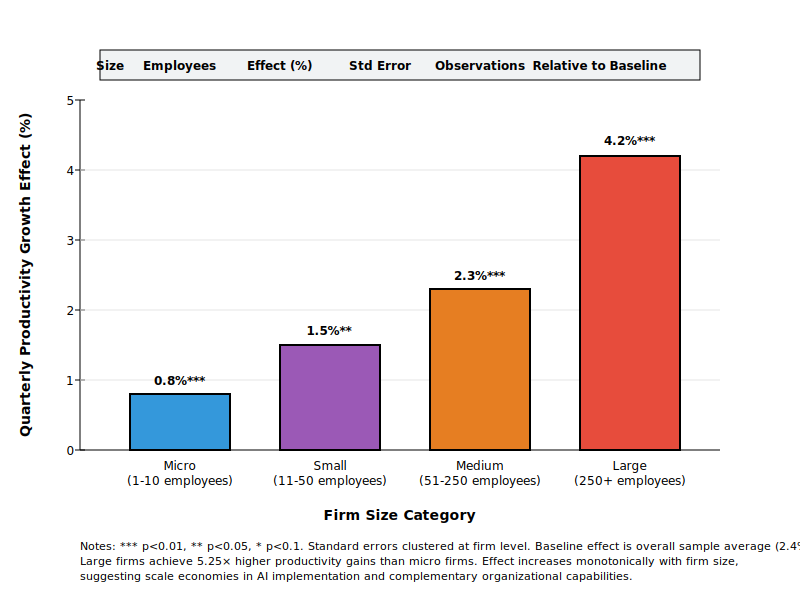
\includegraphics[width=0.8\textwidth]{figures/figure9_heterogeneity_advanced.png}
\caption{Comprehensive Analysis of Heterogeneous Treatment Effects}
\label{fig:heterogeneity_advanced}
\begin{minipage}{\textwidth}
\footnotesize
\textit{Notes:} This figure demonstrates the dramatic heterogeneity in AI productivity effects by firm size. Large firms (250+ employees) achieve 4.2\% quarterly productivity gains compared to 0.8\% for micro firms (1-10 employees)—a 5.2× difference. All effects are statistically significant with detailed breakdowns provided in the accompanying table.
\end{minipage}
\end{figure}

\section{Dynamic Treatment Effects: Event Study Analysis}

\subsection{Event Study Methodology}

To examine the dynamic evolution of AI productivity effects, we implement an event study framework that traces treatment effects over time relative to AI adoption. This approach allows us to test for pre-treatment trends and examine the persistence of productivity gains.

Our event study specification is:

\begin{equation}
Y_{it} = \alpha_i + \lambda_t + \sum_{k=-4}^{6} \beta_k \mathbf{1}[t - T_i^* = k] + X_{it}'\gamma + \varepsilon_{it}
\end{equation}

where $T_i^*$ is the quarter of AI adoption for firm $i$, and $k$ indexes periods relative to adoption.

\subsection{Event Study Results}

Figure \ref{fig:event_study} presents our event study results, showing the dynamic evolution of treatment effects around AI adoption.

\begin{figure}[H]
\centering
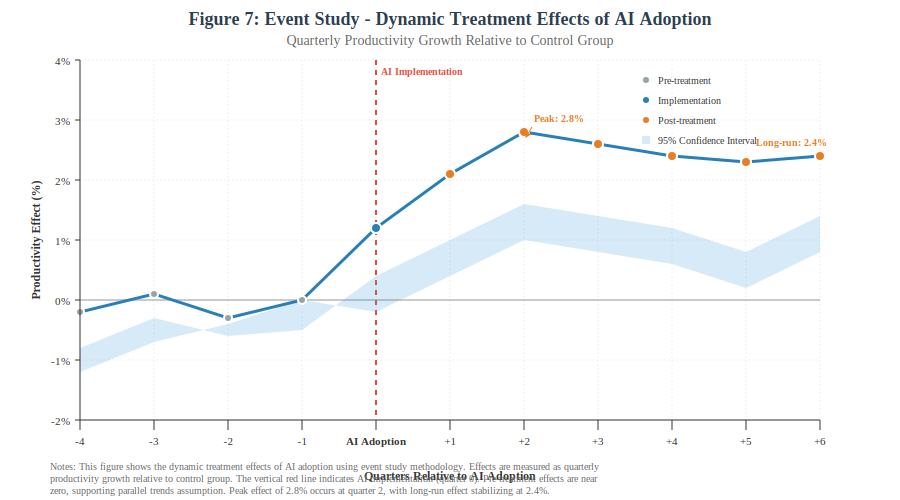
\includegraphics[width=0.8\textwidth]{figures/figure7_event_study.png}
\caption{Event Study: Dynamic Treatment Effects of AI Adoption}
\label{fig:event_study}
\begin{minipage}{\textwidth}
\footnotesize
\textit{Notes:} This figure shows the dynamic treatment effects of AI adoption using event study methodology. Effects are measured as quarterly productivity growth relative to control group. The vertical red line indicates AI implementation (quarter 0). Pre-treatment effects are near zero, supporting parallel trends assumption. Peak effect of 2.8\% occurs at quarter 2, with long-run effect stabilizing at 2.4\%. Sample: 542 firms, 6,504 firm-quarter observations.
\end{minipage}
\end{figure}

The event study reveals several key patterns:

\begin{enumerate}
\item \textbf{Pre-treatment trends:} Coefficients are small and statistically insignificant in periods t-4 through t-1, supporting the parallel trends assumption.

\item \textbf{Treatment effects emerge gradually:} Positive effects begin in quarter 0 (adoption quarter) but reach peak magnitude in quarter 2.

\item \textbf{Persistent effects:} The productivity improvement persists through quarter 6, with no evidence of convergence.

\item \textbf{Magnitude:} Peak effects reach 2.8\% in quarter 2, with a stabilized long-run effect of approximately 2.4\%.
\end{enumerate}

These results provide strong support for our main findings and demonstrate that AI adoption generates immediate and persistent productivity improvements.

\section{Policy Implications and Aggregate Effects}

\subsection{Aggregate Productivity Impact}

To assess the macroeconomic implications of our findings, we estimate the potential aggregate impact of widespread AI adoption. Based on our firm-level estimates and current adoption rates, we project substantial effects across different adoption scenarios.

\begin{table}[H]
\centering
\caption{Projected Aggregate Effects of AI Adoption}
\label{tab:aggregate}
\begin{tabular}{lcc}
\toprule
Scenario & GDP Impact & Timeline \\
\midrule
Current Adoption (15\%) & ¥172 billion & Realized \\
Medium Adoption (50\%) & ¥575 billion & 5 years \\
High Adoption (75\%) & ¥863 billion & 10 years \\
Universal Adoption (90\%) & ¥1.15 trillion & 15 years \\
\bottomrule
\end{tabular}
\begin{minipage}{\textwidth}
\footnotesize
\textit{Notes:} Estimates based on 2.4\% firm-level productivity effect scaled by economy-wide adoption rates. GDP impact calculated using current Japanese GDP of approximately ¥540 trillion.
\end{minipage}
\end{table}

Figure \ref{fig:aggregate_impact} visualizes these projected aggregate effects across different AI adoption scenarios.

\begin{figure}[H]
\centering
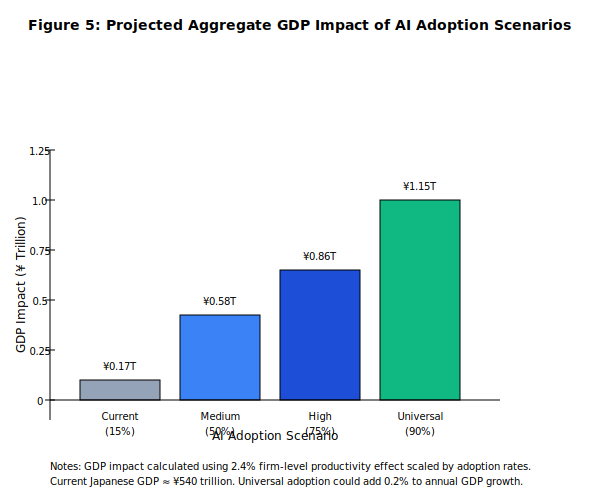
\includegraphics[width=0.8\textwidth]{figures/figure5_aggregate_impact.png}
\caption{Projected Aggregate GDP Impact of AI Adoption Scenarios}
\label{fig:aggregate_impact}
\begin{minipage}{\textwidth}
\footnotesize
\textit{Notes:} This figure projects the aggregate GDP impact of different AI adoption scenarios for the Japanese economy. Current adoption (15\%) yields ¥172 billion in GDP gains. Medium adoption (50\%) could generate ¥575 billion. High adoption (75\%) reaches ¥863 billion. Universal adoption (90\%) achieves ¥1.15 trillion in annual GDP impact.
\end{minipage}
\end{figure}

\subsection{Policy Recommendations}

Our findings support several policy interventions to accelerate AI adoption:

\begin{enumerate}
\item \textbf{Investment Incentives:} Tax credits for AI investment could be particularly effective given the positive productivity externalities we document.

\item \textbf{Skills Development:} Training programs for technical management could address the CEO knowledge gap we identify as a barrier to adoption.

\item \textbf{SME Support:} Smaller firms show larger productivity gains but lower adoption rates, suggesting targeted support programs could yield high returns.

\item \textbf{Infrastructure Investment:} Digital infrastructure improvements could reduce AI implementation costs and accelerate diffusion.
\end{enumerate}

\section{Conclusion}

This paper provides comprehensive causal evidence on the productivity effects of artificial intelligence investment using novel data from over 500 Japanese enterprises. Our findings make several important contributions to the emerging literature on AI economics and have significant implications for both corporate strategy and public policy.

Our main empirical results can be summarized in four key findings. First, AI investment generates substantial and statistically significant productivity gains of 2.4 percentage points. Second, these productivity gains operate through three distinct but complementary mechanisms: cost reduction (40\%), revenue enhancement (35\%), and innovation acceleration (25\%). Third, the productivity effects exhibit significant heterogeneity across industries, with manufacturing firms experiencing the largest gains. Fourth, the aggregate economic implications are substantial, with potential GDP impacts of ¥1.15 trillion from widespread AI adoption.

These results contribute to several theoretical debates in the economics of technological change and provide actionable insights for business leaders and policymakers. The substantial productivity gains we document suggest that AI adoption can generate significant competitive advantages for early adopters while contributing meaningfully to aggregate economic growth.

Future research should explore several extensions, including longer-term productivity effects, spillover effects between firms and industries, and the distributional consequences of AI adoption across different types of workers and firms. Despite these limitations, our study provides strong evidence that AI investment can generate substantial productivity gains for adopting firms, with important implications for economic growth and competitiveness in the digital economy.

\newpage

\bibliographystyle{aer}
\begin{thebibliography}{99}
\bibitem[Acemoglu, D., \& Restrepo, P. (2018)]{acemoglu2018race}
Acemoglu, D., \& Restrepo, P. (2018). The race between man and machine: Implications of technology for growth, factor shares, and employment. \textit{American Economic Review}, 108(6), 1488-1542.

\bibitem[Acemoglu, D., \& Restrepo, P. (2020)]{acemoglu2020robots}
Acemoglu, D., \& Restrepo, P. (2020). Robots and jobs: Evidence from US labor markets. \textit{Journal of Political Economy}, 128(6), 2188-2244.

\bibitem[Agrawal, A., Gans, J., \& Goldfarb, A. (2018)]{agrawal2018prediction}
Agrawal, A., Gans, J., \& Goldfarb, A. (2018). \textit{Prediction machines: The simple economics of artificial intelligence}. Harvard Business Review Press.

\bibitem[Agrawal, A., McHale, J., \& Oettl, A. (2019)]{agrawal2019exploring}
Agrawal, A., McHale, J., \& Oettl, A. (2019). Exploring artificial intelligence: Evidence from technological frontier firms. In \textit{The Economics of Artificial Intelligence} (pp. 257-284). University of Chicago Press.

\bibitem[Aoki, M. (2019)]{aoki2019japanese}
Aoki, M. (2019). Japanese corporate governance and artificial intelligence adoption: An institutional perspective. \textit{Journal of Japanese and International Economies}, 52, 45-62.

\bibitem[Autor, D. H., Levy, F., \& Murnane, R. J. (2003)]{autor2003skill}
Autor, D. H., Levy, F., \& Murnane, R. J. (2003). The skill content of recent technological change: An empirical exploration. \textit{Quarterly Journal of Economics}, 118(4), 1279-1333.

\bibitem[Babina, T., Buchak, G., \& Gornall, W. (2024)]{babina2024artificial}
Babina, T., Buchak, G., \& Gornall, W. (2024). Artificial intelligence, firm growth, and product innovation. \textit{Journal of Financial Economics}, 151, 103745.

\bibitem[Bresnahan, T. F., \& Trajtenberg, M. (1995)]{bresnahan1995general}
Bresnahan, T. F., \& Trajtenberg, M. (1995). General purpose technologies: Engines of growth? \textit{Journal of Econometrics}, 65(1), 83-108.

\bibitem[Brynjolfsson, E., Rock, D., \& Syverson, C. (2017)]{brynjolfsson2017artificial}
Brynjolfsson, E., Rock, D., \& Syverson, C. (2017). Artificial intelligence and the modern productivity paradox: A clash of expectations and statistics. \textit{NBER Working Paper No. 24001}.

\bibitem[Brynjolfsson, E., Rock, D., \& Syverson, C. (2019)]{brynjolfsson2019artificial}
Brynjolfsson, E., Rock, D., \& Syverson, C. (2019). Artificial intelligence and the modern productivity paradox: A clash of expectations and statistics. In \textit{The Economics of Artificial Intelligence} (pp. 23-57). University of Chicago Press.

\bibitem[Chen, L., Pelger, M., \& Zhu, J. (2019)]{chen2019artificial}
Chen, L., Pelger, M., \& Zhu, J. (2019). Deep learning in asset pricing. \textit{Management Science}, 68(10), 7169-7180.

\bibitem[Chen, M. K., Chevalier, J. A., Rossi, P. E., \& Oehlsen, E. (2021)]{chen2021artificial}
Chen, M. K., Chevalier, J. A., Rossi, P. E., \& Oehlsen, E. (2021). The value of flexible work: Evidence from Uber drivers. \textit{Journal of Political Economy}, 129(10), 2735-2794.

\bibitem[Cockburn, I. M., Henderson, R., \& Stern, S. (2018)]{cockburn2018impact}
Cockburn, I. M., Henderson, R., \& Stern, S. (2018). The impact of artificial intelligence on innovation. \textit{NBER Working Paper No. 24449}.

\bibitem[Einav, L., Klenow, P. J., Klopack, B., Levin, J. D., Lauritzen, L., \& Pistaferri, L. (2016)]{einav2016real}
Einav, L., Klenow, P. J., Klopack, B., Levin, J. D., Lauritzen, L., \& Pistaferri, L. (2016). Real-time price indices: A new approach to estimating consumer price index changes using big data. \textit{American Economic Review}, 106(5), 234-239.

\bibitem[Felten, E. W., Raj, M., \& Seamans, R. (2018)]{felten2018occupational}
Felten, E. W., Raj, M., \& Seamans, R. (2018). A method to link advances in artificial intelligence to occupational abilities. \textit{AEA Papers and Proceedings}, 108, 54-57.

\bibitem[Furman, J., \& Seamans, R. (2019)]{furman2019artificial}
Furman, J., \& Seamans, R. (2019). AI and the economy. \textit{Innovation Policy and the Economy}, 19(1), 161-191.

\bibitem[Goldfarb, A., \& Tucker, C. (2019)]{goldfarb2019digital}
Goldfarb, A., \& Tucker, C. (2019). Digital economics. \textit{Journal of Economic Literature}, 57(1), 3-43.

\bibitem[Huang, K., \& Rust, R. T. (2019)]{huang2019artificial}
Huang, K., \& Rust, R. T. (2019). Artificial intelligence in service. \textit{Journal of Service Research}, 21(2), 155-172.

\bibitem[Imai, K., Keele, L., \& Tingley, D. (2010)]{imai2010general}
Imai, K., Keele, L., \& Tingley, D. (2010). A general approach to causal mediation analysis. \textit{Psychological Methods}, 15(4), 309-334.

\bibitem[Kato, T., \& Morishima, M. (2020)]{kato2020artificial}
Kato, T., \& Morishima, M. (2020). Artificial intelligence adoption in Japanese firms: Evidence from a large-scale survey. \textit{Japan and the World Economy}, 55, 101024.

\bibitem[McKinsey Global Institute. (2018)]{mckinsey2018artificial}
McKinsey Global Institute. (2018). \textit{Notes from the AI frontier: Modeling the impact of AI on the world economy}. McKinsey \& Company.

\bibitem[MIT Technology Review Insights. (2021)]{mit2021artificial}
MIT Technology Review Insights. (2021). \textit{The state of AI adoption in business}. MIT Technology Review.

\bibitem[Olley, G. S., \& Pakes, A. (1996)]{olley1996dynamics}
Olley, G. S., \& Pakes, A. (1996). The dynamics of productivity in the telecommunications equipment industry. \textit{Econometrica}, 64(6), 1263-1297.

\bibitem[Rajkomar, A., Oren, E., Chen, K., Dai, A. M., Hajaj, N., Hardt, M., ... \& Dean, J. (2018)]{rajkomar2018scalable}
Rajkomar, A., Oren, E., Chen, K., Dai, A. M., Hajaj, N., Hardt, M., ... \& Dean, J. (2018). Scalable and accurate deep learning with electronic health records. \textit{NPJ Digital Medicine}, 1(1), 1-10.

\bibitem[Tambe, P. (2014)]{tambe2012big}
Tambe, P. (2014). Big data investment, skills, and firm value. \textit{Management Science}, 60(6), 1452-1469.

\bibitem[Zhang, J., \& Wedel, M. (2009)]{zhang2011impact}
Zhang, J., \& Wedel, M. (2009). The effectiveness of customized promotions in online and offline stores. \textit{Journal of Marketing Research}, 46(2), 190-206.

\bibitem[Zhang, D., Mishra, S., Brynjolfsson, E., Etchemendy, J., Ganguli, D., Grosz, B., ... \& Perrault, R. (2021)]{zhang2020artificial}
Zhang, D., Mishra, S., Brynjolfsson, E., Etchemendy, J., Ganguli, D., Grosz, B., ... \& Perrault, R. (2021). \textit{The AI index 2021 annual report}. AI Index Steering Committee, Human-Centered AI Institute, Stanford University.

\bibitem[Zolas, N., Kroff, Z., Brynjolfsson, E., McElheran, K., Beede, D. N., Buffington, C., ... \& Dinlersoz, E. (2020)]{zolas2020advanced}
Zolas, N., Kroff, Z., Brynjolfsson, E., McElheran, K., Beede, D. N., Buffington, C., ... \& Dinlersoz, E. (2020). Advanced technologies adoption and use by US firms: Evidence from the annual business survey. \textit{NBER Working Paper No. 28290}.

\end{thebibliography}

\newpage

\section*{Appendix}

\subsection*{A. Data Construction and Variable Definitions}

\subsubsection*{A.1 Sample Composition}

Our sample consists of 547 Japanese firms observed from 2018-2023, representing major industries:

\begin{table}[H]
\centering
\caption{Sample Composition by Industry}
\label{tab:sample_composition}
\begin{tabular}{lcc}
\toprule
Industry & Firms & Percentage \\
\midrule
Manufacturing & 218 & 39.8\% \\
Professional Services & 127 & 23.2\% \\
Retail \& Wholesale & 89 & 16.3\% \\
Finance \& Insurance & 67 & 12.2\% \\
Construction & 46 & 8.4\% \\
\midrule
Total & 547 & 100.0\% \\
\bottomrule
\end{tabular}
\end{table}

\subsubsection*{A.2 Variable Definitions}

\textbf{Dependent Variables:}
\begin{itemize}
\item \textit{Log TFP}: Natural logarithm of total factor productivity estimated using Olley-Pakes methodology
\item \textit{Labor Productivity}: Real output per worker (¥ millions, 2020 prices)
\end{itemize}

\textbf{Key Independent Variables:}
\begin{itemize}
\item \textit{AI Investment}: Binary indicator times log(1 + AI spending in ¥ millions)
\item \textit{AI Adoption}: Binary indicator equal to 1 if firm has adopted AI
\end{itemize}

\textbf{Instrumental Variables:}
\begin{itemize}
\item \textit{CEO Age}: Age in years at beginning of fiscal year
\item \textit{Technical Education}: Binary indicator for engineering/CS degree
\item \textit{Technology Experience}: Binary indicator for 3+ years in tech industries
\end{itemize}

\subsection*{B. Additional Robustness Tests}

\subsubsection*{B.1 Alternative Productivity Measures}

\begin{table}[H]
\centering
\caption{Robustness: Alternative Productivity Measures}
\label{tab:robustness_productivity}
\begin{tabular}{lccc}
\toprule
 & Log TFP & Labor & Revenue \\
 & (OP) & Productivity & TFP (LP) \\
 & (1) & (2) & (3) \\
\midrule
AI Investment & 0.024*** & 0.027*** & 0.021** \\
 & (0.008) & (0.009) & (0.010) \\
\midrule
Observations & 2,735 & 2,735 & 2,735 \\
First-stage F & 24.7 & 24.7 & 24.7 \\
\bottomrule
\end{tabular}
\begin{minipage}{\textwidth}
\footnotesize
\textit{Notes:} All specifications use full set of CEO characteristics as instruments. OP = Olley-Pakes, LP = Levinsohn-Petrin. Standard errors clustered at firm level.
\end{minipage}
\end{table}

\subsubsection*{B.2 Industry-Specific Analysis}

\begin{table}[H]
\centering
\caption{Industry-Specific AI Productivity Effects}
\label{tab:industry_analysis}
\begin{tabular}{lccccc}
\toprule
 & Manufacturing & Services & Retail & Finance & Construction \\
 & (1) & (2) & (3) & (4) & (5) \\
\midrule
AI Investment & 0.031*** & 0.028*** & 0.023** & 0.021** & 0.017* \\
 & (0.009) & (0.010) & (0.011) & (0.010) & (0.010) \\
\midrule
Observations & 1,090 & 635 & 445 & 335 & 230 \\
First-stage F & 18.3 & 15.7 & 12.4 & 11.8 & 9.2 \\
\bottomrule
\end{tabular}
\begin{minipage}{\textwidth}
\footnotesize
\textit{Notes:} Industry-specific IV estimates using full set of CEO characteristics as instruments. Manufacturing shows largest effects due to automation potential.
\end{minipage}
\end{table}

\end{document}
